\chapter{Signal Uncertainty: Estimation and Sampling} % Main chapter title

\label{chap:variance} % Change X to a consecutive number; for referencing this chapter elsewhere, use \ref{ChapterX}

\lhead{Chapter 5. \emph{Signal Uncertainty: Estimation and Sampling}} % 

So far in this thesis we have introduced several Bayesian GSP models and focused on tractable methods for finding mean of the associated Gaussian posterior. In this chapter, we turn our attention to the posterior \textit{covariance}, which presents several new interesting challenges. These challenges stem from the dimensionality the associated covariance matrix which, in each case, is the inverse of a large Kronecker-structured operator. For example, consider the two-dimensional graph signal reconstruction problem defined in \cref{sec:gsr_cpg}. The posterior mean has shape $(N \times T)$ and the posterior covariance matrix has shape $(NT \times NT)$. For a modest-sized problem comprising a 200-node graph measured over 365 time points, the (known) precision matrix will have over $5 \times 10^9$ elements, corresponding to over 20GB of memory with 32-bit floating-point numbers. Even if this could be held in RAM, inverting a matrix of this size would be intractable on consumer-grade hardware. This problem is only compounded when considering the tensor-valued models introduced in \cref{chap:nd_gsp}, where the covariance matrices have $O(N^2)$ elements, where $N = \prod N_i$. \Cref{tab:post_cov} lists the posterior covariance matrices that appear in these models, along with their associated dimensionality. 

\setcellgapes{8pt}
\makegapedcells

\begin{table}[hb]
    \def\arraystretch{1.5}
    \centering
    \begin{tabular}{|c|c|c|}
    \hline
    \textbf{Model} & \textbf{Covariance matrix} & \textbf{Element count}\\
    \hline
    GSR & $\left(\D_{\St} + \gamma \HH^{-2}\right)^{-1}$ & $ \prod N_i^2 $\\ 
    \hline
    KGR & $\left(\D_{\St} + \gamma \K^{-1} \otimes \HH^{-2}\right)^{-1}$ & $T^2\prod N_i^2$\\ 
    \hline
    RNC & $\begin{bmatrix}
        \D_\St + \gamma \HH^{-2} & \D_\St  \X \\
        \X^\top \D_\St & \X^\top \D_\St \X + \lambda \I_M   
       \end{bmatrix}^{-1}$ & $\Big(\prod N_i + M\Big)^2$ \\ 
    \hline
    KG-RNC & $\begin{bmatrix}
        \D_\St + \gamma \K^{-1} \otimes \HH^{-2} & \D_\St  \X \\
        \X^\top \D_\St & \X^\top \D_\St \X + \lambda \I_M   
       \end{bmatrix}^{-1}$ & $\Big(T\prod N_i + M\Big)^2$ \\
    \hline
\end{tabular}
\caption{The posterior covariance matrix appearing in the tensor GSR, KGR, RNC and KR-RNC models.  }
\label{tab:post_cov}
\end{table}

\setcellgapes{2pt}


Given these challenges, the goal of this chapter is to to gain insight into the uncertainty about the predicted posterior mean, whilst circumventing the need to instantiate, invert or decompose large matrices directly in memory. To this end, we specify two separate but related tasks of interest:

\begin{enumerate}
    
    \item \textit{To estimate the posterior marginal variance}. Given a large, known precision matrix with a Kronecker structure, the task is to estimate the diagonal of the associated covariance matrix (its inverse). Whilst the most straightforward approach would be simply to invert the precision matrix directly and take the diagonal, this will be too memory intensive for most practical applications. Computing the marginal variance alone disregards information about the correlation between elements, but still gives valuable insight into prediction uncertainty whilst remaining tractable to store in memory. Therefore, the first task is to produce a scalable algorithm for estimating the diagonal of the posterior covariance matrix. 
    \item \textit{To sample directly from the posterior}. For many applications, the ability to draw independent samples directly from the posterior is of significant interest. However, due to the size of the relevant matrices, direct Cholesky decomposition approaches will be intractable for most realistic use cases. Therefore, the second task is to produce an algorithm that can efficiently draw independent random samples from the posterior, whilst avoiding the memory and computational difficulties associated with the most straightforward approaches. 
\end{enumerate}

The chapter is structured as follows. First, in \cref{sec:post_var_pred}, we consider different approaches for estimating the posterior marginal variance. In particular, we compare a recent stochastic technique for estimating a matrix diagonal \citep{Bekas2007, Tang2012} with several custom regression models which leverage intuition about the network structure of the problem. We show that, by including these network effects, our method significantly outperforms the aforementioned stochastic technique on a test dataset. Next, in \cref{sec:sampling}, we make use of a recently proposed technique for direct sampling known as Perturbation Optimisation (PO) \citep{Vono2022}. PO is relevant when the precision matrix can be split into a sum of matrices with a known eigenvalue decomposition which, as we will show, is always the case in our models. This allows us to draw independent samples from the posterior distribution for the same computational cost as is required to calculate the posterior mean which, as established in \cref{chap:nd_gsp}, can be achieved efficiently using iterative methods. 

The methods derived in this chapter are designed to be applicable to tensor-valued GSP problems covered in \cref{chap:nd_gsp}. However, since the two-dimensional methods covered in \cref{chap:gsr_2d,chap:kgr_rnc_2d} can be considered special cases of the more general MWGSP format, these too are included under the same framework. 

\section{Estimating the posterior marginal variance}

\label{sec:post_var_pred}

Consider the multiway Graph Signal Reconstruction problem as defined in \cref{chap:nd_gsp}. Here, the goal is to estimate a smooth underlying signal, $\Ft$, with shape $(N_1, N_2, ..., N_d)$, given a partially observed graph signal, $\Yt$, and binary sensing tensor, $\St$, both of which have the same shape as $\Ft$. In \cref{sec:tensor_gsr}, we demonstrate that the posterior distribution over $\f \in \R^N = \vecrm{\Ft}$, given $\y \in \R^N  = \vecrm{\Yt}$, is

\begin{equation}
    \f \, | \, \y \sim \Norm{\PP^{-1} \y}{\PP^{-1}}
\end{equation}

where 

\begin{equation}
    \label{eq:P_posterior}
    \PP \in \R^{N \times N} = \D_{\St} + \gamma \HH^{-2}
\end{equation}

The goal of this section is to estimate the diagonal of the covariance matrix $\PP^{-1}$ without directly evaluating the matrix in full. For the sake of brevity, we focus on estimating the posterior marginal variance for the GSR model alone in this section. However, the methods discussed can easily be generalised to KGR, RNC and KG-RNC by making suitable modifications. 

\subsection{A baseline approach}

\label{sec:var_baseline}

As previously established, it is possible to efficiently solve a linear system of the form $\PP^{-1} \z$, where $\z$ is an arbitrary length-$N$ vector, using the SIM or CGM. Therefore, a straightforward approach to computing the marginal variance in full is immediately available: to compute the $n$-th column of $\PP^{-1}$, we can solve the linear system $\PP^{-1} \e_n$, where $\e_n$ is the $n$-th unit basis vector. Consequently, to compute the entire marginal variance in full, we solve this system $N = \prod N_i$ times, once for each $n \in [1, 2, ..., N]$, retaining only the $n$-th element of the resultant solution each time.
    
Whilst this strategy has lower time and memory complexity than performing direct inversion of $\PP$, it still presents significant computational challenges. Since obtaining each element of the marginal variance necessitates solving a linear system, the whole process takes $N$ times longer than the computation of the mean, which itself can be intensive for large problems. It is clear that this approach is not scalable. A natural question, then, is whether the full marginal variance can be \textit{estimated} for a lower computational cost. 


\subsection{Matrix diagonal estimation}

\label{sec:logvar_bekas}

One notable recent approach for estimating the diagonal of an arbitrary matrix comes from \cite{Bekas2007}, which was subsequently updated in \cite{Tang2012}. Here, the authors propose a stochastic technique, based on the earlier work of \cite{Hutchinson1990}, which was designed to estimate the trace of a matrix. The authors define the estimator for $\diag{\PP^{-1}}$ as follows. 
 
\begin{equation}
    \label{eq:bekas}
    \diag{\PP^{-1}} \approx \left(\sum_{r=1}^R \ve_r \circ \PP^{-1} \ve_r \right) \oslash \left(\sum_{k=1}^s \ve_r \circ \ve_r \right)
\end{equation}

Here, $\oslash$ denotes element-wise division, and $\circ$ is the Hadamard product (element-wise multiplication) as before. In the original specification, the vectors $\{\ve_r\}$ have entries of $\pm 1$ which are drawn uniformly at random. This estimator converges to the true diagonal of $\PP^{-1}$ as $R \rightarrow \infty$ \citep{Bekas2007}. For this technique to be scalable, it is necessary for the system $\PP^{-1} \ve$ to be solved efficiently for an arbitrary vector $\ve$ (which it can in our case, using the SIM or CGM). Furthermore, the algorithm requires $\PP^{-1} \ve$ to be computed for $R$ different values of $\ve_r$. Therefore the overall complexity of this approach is proportional to $R$. For this estimator to be better than the baseline approach outlined in \cref{sec:var_baseline}, we must reach an acceptable level of accuracy for $R \ll N$. 


\subsection{A supervised learning approach}

In this subsection we introduce the key contribution of the first half of this chapter. The basic idea is as follows. Using the approach outlined in \cref{sec:var_baseline}, we can compute the `true' variance at a limited number, $Q$, of the elements by solving the linear system $\PP^{-1}\e_n$, and retaining only the $n$-th element of the resultant vector, for a set of elements $\mathcal{Q}$. Next, we \textit{predict} the the marginal variance at all the other elements not in the set $\mathcal{Q}$. If we can construct a set of artificial explanatory variables associated with each element, then this becomes a standard supervised learning problem. 

Since variance is strictly positive, we choose to predict the \textit{log}-variance rather than the variance itself. This transformation changes the prediction range from the positive values of $[0, \infty]$ to the full range of $[-\infty, \infty]$, which is more suitable for standard regression techniques. We define the target variable, denoted as $\Omegat$, as follows.

\begin{equation}
    \Omegat \in \R^{N_1 \times N_2 \times ... \times N_d} = \tenrm{\text{log}\left(\diagi{\PP^{-1}}\right)}
\end{equation}

Note that here we have introduced the notation $\diagi{\cdot}$, which denotes a function mapping the diagonal of an $(N \times N)$ matrix into a length-$N$ vector. Therefore, the whole expression can be understood as taking the diagonal of the covariance matrix $\PP^{-1}$, performing an element-wise logarithm, and transforming this into a tensor, $\Omegat$,  of shape $(N_1, N_2, ..., N_d)$ in row major order. The objective of the regression algorithms discussed in this section is to predict the tensor $\Omegat$.

To make this prediction, we first compute a subset of the elements of $\Omegat$. Since $\Omegat$ is an order-$d$ tensor, its elements are indexed by a length-$d$ integer vector, $\nn$. Therefore we can describe the indices that we choose to compute by the set $\mathcal{Q} = \{\nn_1, \nn_2, ..., \nn_Q \}$. Additionally, we define the binary tensor $\Qt$, which also indicates which elements of $\Omegat$ have been computed. 

\begin{equation}
    \Qt_{\nn} = \begin{cases}
        1 & \text{if} \;\; \nn \in \mathcal{Q} \\
        0 & \text{otherwise}
    \end{cases}
\end{equation}


For each index $\nn$, the corresponding element of $\Omegat$ can be computed as 

\begin{equation}
    \Omegat_\nn = \tenrm{\log \left( \PP^{-1} \e_n \right)}_{\nn}
\end{equation}

For a vector index $\nn = [n_1, n_2, ..., n_d]$, the corresponding unit vector $\e_n$ is 

\begin{equation}
\e_n = \e_{n_1} \otimes \e_{n_2} \otimes ... \otimes \e_{n_d}
\end{equation}

The linear system $\PP^{-1} \e_n$ can then be solved efficiently using either the tensor SIM or CGM as discussed in \cref{sec:SIM_dd,sec:CGM_dd}. We refer to the process of computing these elements of $\Omegat$ as \textit{querying}. The result, after $Q$ queries, is a partial observation of the matrix $\Omegat$, where $Q$ of its entries have been filled in, and the rest are set to zero. We refer to this tensor as $\Omegat_Q$. 


\begin{equation}
    \Omegat_Q = \Qt \circ \Omegat
\end{equation}

As mentioned, we also need a set of explanatory variables to help predict the unknown elements of $\Omegat$. In particular, every element, $\nn$, should have an associated feature vector, $\x_\nn$, which should have some explanatory power over $\Omegat_\nn$. In this way, the problem becomes a regular supervised learning task where the goal is to predict $\Omegat$ given the labelled training pairs $\{\Omegat_\nn, \x_\nn\}_{\nn \in \mathcal{Q}}$. If each feature vector has length $k$, the explanatory variables as a whole can be described by the tensor $\Xt$ with shape $(N_1, ..., N_d, k)$. The question then becomes how to construct the tensor $\Xt$ such that it is likely to explain the posterior marginal variance well. 

By inspecting \cref{eq:P_posterior}, it is clear that the marginal variance can only depend on $\St$, and $\HH$, since these are the only matrices appearing in the posterior covariance ($\gamma$ can be considered a constant for the purpose of this problem). $\HH$ itself also depends on the graph filter used and the structure of the graph. Therefore, we should choose features which capture different aspects of these objects. 

\begin{table}[t]
    \renewcommand{\arraystretch}{1.7}
    \centering
    \begin{tabular}{|c|c|c|c|}
    \hline
     & \textbf{Description} & \textbf{Representation}\\
    \hline
    $\Xt_{:,1}$ &  Constant & $\mathbf{1}_{(N_1, N_2, ..., N_d)}$ \\
    \hline
    $\Xt_{:,2}$ & Missing observations & $\St'$  \\
    \hline
    $\Xt_{:,3}$ & Missing obs filtered & $\text{IGFT} \Big(\Gt \circ \text{GFT}\big(\Xt_{:,2}\big)\Big)$ \\
    \hline 
    $\Xt_{:,4}$ &  Diagonal of $\HH$ & $\tenrm{\diagi{\HH}}$ \\
    \hline 
    $\Xt_{:,5}$ & Diagonal of $\HH^2$ & $\tenrm{\diagi{\HH^2}}$ \\
    \hline
    $\Xt_{:,6}$ &  N-neighbours & $\tenrm{\A \mathbf{1}_N}$\\
    \hline
    $\Xt_{:,7}$  & N-neighbours filtered &  $\text{IGFT} \Big(\Gt \circ \text{GFT}\big(\Xt_{:,6}\big)\Big)$ \\
    \hline
\end{tabular}
\caption{\small{The explanatory variables used to predict the posterior log-variance. Note that $\Xt_{:,4}$ and $\Xt_{:,5}$ have an efficient computation - see \cref{the:efficient_H_diag} }}
\label{tab:post_cov_features}
\end{table}


In the following, we use $k=7$ different descriptors which are summarised in \cref{tab:post_cov_features}. For the features that include a filtering operation ($\Xt_{:,3}$ and $\Xt_{:,7}$), we use the same filter parameters that were used in the original GSR specification. As in the RNC model of \cref{sec:rnc_dd}, we can combine these tensor variables together into a single matrix $\X$ as follows. 

\begin{equation}
    \X \in \R^{N \times 7} = \begin{bmatrix} \vecrm{\Xt_{:, 1}} & \vecrm{\Xt_{:, 2}} & \dots & \vecrm{\Xt_{:, 7}} \end{bmatrix}    
\end{equation}



\subsubsection{Solving with Ridge Regression}

\label{sec:logvar_RR}

The first strategy we use to predict the posterior log-variance is simply ridge regression. Here, we model the posterior log-variance $\Omegat$ as a linear combination of the features given in \cref{tab:post_cov_features}, with the optimal weighting, $\w$, learned from the observed data. In particular, the predicted value of $\Omegat$, which we label $\Omegat^\star$ is given simply by 

$$
\Omegat^\star = \tenrm{\X \w^\star}
$$

where 

$$
\w^\star = \left(\X^\top \D_\Qt \X + \lambda \I_N\right)^{-1} \X^\top  \vecrm{\Omegat_Q}
$$

Note that since $\D_\Qt = \diag{\vecrm{\Qt}}$ is a sparse diagonal matrix, the product $\X^\top \D_\Qt \X$ can be computed efficiently with $O(k^2Q)$ operations. This model includes a regularisation parameter $\lambda$ which must be set ahead of time (or potentially learned via cross validation).


\subsubsection{Solving with RNC}

\label{sec:logvar_RNC}

The next strategy we use to predict the marginal variance is tensor Regression with Network Cohesion (RNC), as set out in \cref{sec:rnc_dd}. This extends ridge regression by including a flexible intercept term, $\Ct$, which is assumed to be smooth with respect to the graph topology. Since we expect that posterior uncertainty should propagate via closely connected nodes, it is reasonable to assume that $\Omegat$ varies smoothly over the network. In this case, the predicted value for $\Omegat$ is given by 


\begin{equation}
    \Omegat^\star = \Ct^\star + \tenrm{\X \w^\star}
\end{equation}

where

\begin{equation}
    \begin{bmatrix}
        \vecrm{\Ct^\star} \\ \w^\star 
    \end{bmatrix} = \begin{bmatrix}
        \D_\Qt + \gamma \HH^{-2} & \D_\Qt \X \\
        \X^\top \D_\Qt & \X^\top \D_\Qt \X + \lambda \I_7
    \end{bmatrix}^{-1} \begin{bmatrix}
        \vecrm{\Omegat_Q} \\ \X^\top \vecrm{\Omegat_Q}
    \end{bmatrix}
\end{equation} 


Once again, this linear system can be solved efficiently using the SIM or CGM as discussed in \cref{sec:rnc_dd}. 


\subsubsection{Ridge regression with learned filter parameters}

\label{sec:logvar_LFP}

The final novel method we consider for prediction of the posterior log-variance is based on the empirical observation that the predictions made by ridge regression can be improved by adjusting the parameters that characterise the graph filter used to construct features $\Xt_{:,3}$ and $\Xt_{:,7}$. However, it is difficult to tell ahead of time the direction and magnitude of the optimal adjustment. For this reason, we propose a new estimator for $\Omegat$ that simultaneously learns the coefficients multiplying each feature in \cref{tab:post_cov_features}, as well as the filter parameters characterising $\Xt_{:, 3}$ and $\Xt_{:, 7}$, which can vary independently. This can be expressed as follows. 

\begin{equation}
    \Omegat^\star = \tenrm{\X(\betaa^\star) \w^\star}
\end{equation}

Note that now $\X$ is a function of the filter parameters $\betaa$. In order to find the optimal values for both $\w^\star$ and $\betaa^\star$, we use the following loss function. 

\begin{equation}
    \label{eq:LFP_loss}
    \xi(\w, \betaa) = || \Omegat_Q - \Qt \circ \tenrm{\X(\betaa) \w} ||^2_F + \lambda \left(||\w||^2 + ||\betaa - \betaa_0 ||^2\right)
\end{equation}


where $\betaa_0$ represents the parameters characterising the original graph filter in the base GSR problem. Minimising the expression in \cref{eq:LFP_loss} is in general a non-convex optimisation problem. However, a reasonable initial estimate for $\w$ is easily attainable by solving the ridge regression problem. From there, only minor adjustments are necessary for significant improvement in predictive performance. Therefore, off-the-shelf nonlinear optimisation algorithms such as quasi-Newton methods like BFGS can be readily applied \citep{Fletcher2013}. 


\subsection{Query strategies}

\label{sec:query_strats}

So far in this discussion we have not addressed the question of how to select which elements of $\Omegat$ to query. The simplest approach is to uniformly select samples at random. However, although unbiased, this can lead to a high variance estimator, particularly when the query size is very small. A preferable approach is to select elements in a principled way, such that the variance of the estimator is reduced for a small sample size. This is likely to be achieved when the associated features of the samples are representative of the population at large. 

Here we make use of a simple but effective query strategy. First, cluster the elements $\{ \nn \}$ into $K \leq Q$ groups based on the data matrix $\X$. Any clustering algorithm can be used here: a simple and fast option is $K$-means \citep{MacQueen1967, Hartigan1979}. Next, generate a query set $\mathcal{Q}$ by randomly choosing a new data point from each cluster in order. This simple approach is made explicit in \cref{al:K_means}. 

\begin{algorithm}[t]
\begin{algorithmic}
\vspace{0.05cm}
\Require{Number of clusters $K$} 
\vspace{0.05cm}
\Require{Number of queries $Q$} 
\vspace{0.05cm}
\Require{Data matrix $\X \in \R^{N \times 7}$} 
\vspace{0.15cm}
\State{Group data into $K$ randomly ordered cluster sets $\{\mathcal{C}_k\}_{k=1}^{K}$ using $K$-means algorithm}
\vspace{0.15cm}
\State{Create empty query set $\mathcal{Q}$}
\vspace{0.15cm}
\For{$q$ from 1 to $Q$}
\vspace{0.15cm}
\State{Select next non-empty cluster set $\mathcal{C}$}
\vspace{0.15cm}
\State{Choose member $n_q$ from cluster set $\mathcal{C}$ at random}
\vspace{0.15cm}
\State{Add member $n_q$ to query set $\mathcal{Q}$ }
\vspace{0.15cm}
\State{Remove member $n_q$ from cluster set $\mathcal{C}$}
\vspace{0.15cm}
\EndFor
\vspace{0.15cm}
\Ensure{ Query set $\mathcal{Q}$}
\vspace{0.15cm}
\end{algorithmic}
\caption{Querying based on representative samples}
\label{al:K_means}
\end{algorithm}


\subsection{Comparison and analysis}

\label{sec:logvar_experiments} 

In order to compare the performance of the various techniques discussed in this section, we ran the following simple experiment which was setup as follows. First, a product graph was generated by taking the Cartesian product of three random connected graphs, with 10, 15 and 20 nodes respectively, resulting in a graph with $10 \times 15 \times 20 = 3000$ total nodes. Next, we generated a random binary sensing tensor $\St$ of shape $(10, 15, 20)$ by setting elements to zero or one uniformly at random. Finally, we chose a anisotropic diffusion graph filter with $\betaa = [0.5, 0.7, 0.6]$, and set $\gamma$ to one. The task, then, was to predict the diagonal of $(\D_\St + \gamma \HH^{-2})^{-1}$ given the values as specified. Given the relatively small size of the problem, we could compute the true value of $\Omegat$ by running the baseline algorithm as discussed in \cref{sec:var_baseline} over 3000 elements. 

Next, we compared the performance of each of the algorithms discussed in this section. They were the traditional diagonal estimation algorithm of \cite{Bekas2007} (Bekas) outlined in \cref{sec:logvar_bekas}, Ridge Regression (RR), as outlined in \cref{sec:logvar_RR}, Regression with Network Cohesion (RNC) as outlined in \cref{sec:logvar_RNC}, and finally ridge regression with Learned Filter Parameters (LFP), as outlined in \cref{sec:logvar_LFP}. For each strategy, we measured the performance of the estimator by computing the total square error of the predicted variance (not the log-variance), and the $R^2$ statistic of the predicted variance. To be explicit, these were calculated as follows. 

\begin{equation}
    \text{Square error} = || \exp(\Omegat) - \exp(\Omegat^\star)||_F^2
\end{equation}

\begin{equation}
    R^2 = 1 - \frac{|| \exp(\Omegat) - \exp(\Omegat^\star)||_F^2}{ \raisebox{-0.1cm} { $|| \exp(\Omegat) - \overline{\exp(\Omegat)}||_F^2$ }}
\end{equation}

where $\overline{\exp(\Omegat)}$ means the mean of $\exp(\Omegat)$ across all elements. For the case of the Bekas estimator, there was no need to exponentiate the prediction, since it estimates the posterior variance directly, not the log-variance. 

For each of these different estimators, we measured the performance via these two metrics across a range of values of $Q$, i.e. for different numbers of queries. In the case of the Bekas estimator, we measured the performance for different values of $R$ [see \cref{eq:bekas}]. Since each query requires solving the linear system $\PP^{-1}\e_n$, and each iteration of the Bekas algorithm requires solving the linear system $\PP^{-1}\ve_r$, these two measures have a direct correspondence in terms of total compute time. 

For the case of RR, RNC and LFP, we also compared the performance when using a random query strategy, and the representative sampling query strategy as outlined in \cref{al:K_means}. The results are shows in \cref{fig:var_solvers}. On the $x$-axis, we show the number of queries (number of Bekas iterations) as a percentage of the total number of elements, i.e. $Q/N$ (or $R/N$ for Bekas). 


\begin{figure}[t] 
    \begin{center}
        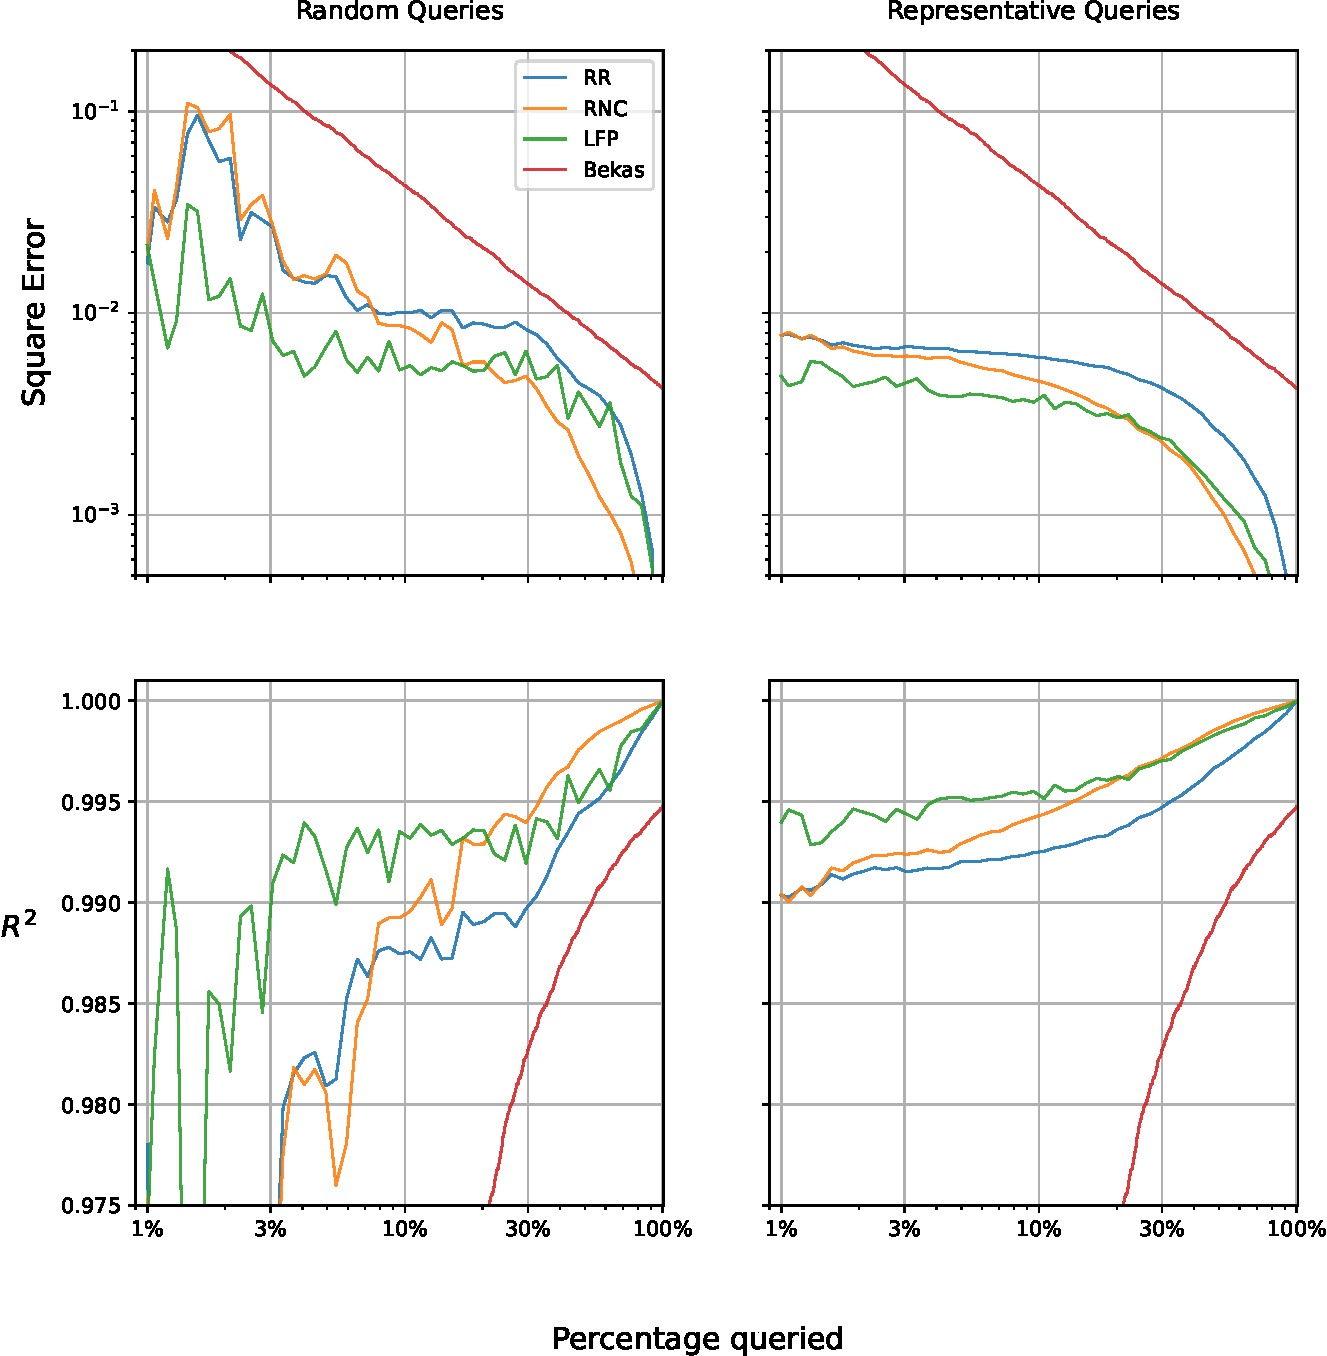
\includegraphics[width=\linewidth]{Figures/VarSolvers.pdf}
    \end{center}
   \caption[Performance of various algorithms for predicting the posterior log-variance]{The performance of the various algorithms for predicting the posterior log-variance is shown as a function of the percentage of $\Omegat$ that has been queried. The top row shows the total square error of the posterior variance, and the bottom row shows the $R^2$ statistic. The left column shows results for random queries and the right column show the results when using representative queries as outlined in \cref{al:K_means}. Since the Bekas technique does not depend on this algorithm, it is repeated in the left and right columns for reference. } 
    \label{fig:var_solvers}
\end{figure} 

The results show that the three supervised learning-based strategies (RR, RNC and LFP) all significantly out-perform Bekas on this synthetic dataset. Moreover, when coupled with the representative sampling strategy of \cref{al:K_means}, all three achieve an $R^2$ statistic of around 0.99 when only 1\% of the elements of $\Omegat$ are queried. These results clearly demonstrate the value of this sampling strategy, especially when the number of queries is low. On this dataset, \cref{al:K_means} has a significant positive impact on performance up to a query percentage of around 3\%, beyond which the difference is less pronounced. 

Of the three supervised learning-based techniques, LFP tends to display the strongest performance at low query percentages, for both random and representative query strategies. RR and RNC have similar performance in this domain, with RNC improving more as the query percentage increases. 

Overall, these results demonstrate that high accuracy predictions ($R^2$ of roughly 0.99) can be achieved for a very low query number relative to the total number of nodes $N$, especially when combined with \cref{al:K_means}. While limited to this particular graph signal processing application, the supervised learning strategy is clearly more effective than the more general technique of \cite{Bekas2007} on this dataset. 


\section{Posterior Sampling}

\label{sec:sampling}


In this section we move to the second aim of this chapter which is to produce an algorithm for direct sampling from the posterior. 

This technique has been dubbed Perturbation Optimisation (PO) since it draws perturbed versions of the mean vectors before using them to define the linear system to solve \citep{Papandreou2010, Orieux2012}. 


\subsection{Perturbation optimization}



\section{Estimation vs Sampling}

\label{sec:comparison}

\subsection{Experiments}
